\let\negmedspace\undefined
\let\negthickspace\undefined
\documentclass[journal]{IEEEtran}
\usepackage[a4paper, margin=10mm, onecolumn]{geometry}
\usepackage{lmodern}
\usepackage{tfrupee}
\setlength{\headheight}{1cm}
\setlength{\headsep}{0mm}
\usepackage{gvv-book}
\usepackage{gvv}
\usepackage{cite}
\usepackage{amsmath,amssymb,amsfonts,amsthm}
\usepackage{algorithmic}
\usepackage{graphicx}
\usepackage{float}
\usepackage{textcomp}
\usepackage{xcolor}
\usepackage{txfonts}
\usepackage{listings}
\usepackage{enumitem}
\usepackage{mathtools}
\usepackage{gensymb}
\usepackage{comment}
\usepackage[breaklinks=true]{hyperref}
\usepackage{tkz-euclide}
\usepackage{listings}
\def\inputGnumericTable{}
\usepackage[latin1]{inputenc}
\usepackage{color}
\usepackage{array}
\usepackage{longtable}
\usepackage{calc}
\usepackage{multirow}
\usepackage{hhline}
\usepackage{ifthen}
\usepackage{lscape}
\usepackage{tikz}
\usetikzlibrary{patterns}

\begin{document}

\bibliographystyle{IEEEtran}
\vspace{3cm}

\title{Question 2.8.38}
\author{EE25BTECH11048 - Revanth Siva Kumar D}

\maketitle
{\let\newpage\relax\maketitle}
\renewcommand{\thefigure}{\theenumi}
\renewcommand{\thetable}{\theenumi}
\setlength{\intextsep}{10pt}

\textbf{Question:}
If the direction cosines of a line are $\brak{k,k,k}$, then find the value of $k$.

\textbf{Solution:}
The direction cosines of a line are denoted by $k, k, k$.  
So, the direction cosine vector becomes
\begin{align}
\vec{d} = \myvec{k \\ k \\ k}
\label{eq:dc_condition}
\end{align}
since d is a unit vector \begin{align}
    \norm{d}=1
    \label{eq:norm}
\end{align}

Applying condition \eqref{eq:dc_condition},
\begin{align}
\norm{\myvec{k \\ k \\ k}} &= \norm{d} \\
(from \eqref{eq:norm} \norm{d}=1)\\
\norm{\myvec{k\\k\\k}} &= 1\\
\sqrt{3k^2} &= 1 \\ 
3k^2 &= 1 \\
k^2 &= \frac{1}{3}
\end{align}

Hence,
\begin{align}
k = \pm \frac{1}{\sqrt{3}}
\end{align}

So, the line vectors are
\[
\vec{v}_1 = \myvec{\frac{1}{\sqrt{3}} \\ \frac{1}{\sqrt{3}} \\ \frac{1}{\sqrt{3}}}, 
\quad
\vec{v}_2 = \myvec{-\frac{1}{\sqrt{3}} \\ -\frac{1}{\sqrt{3}} \\ -\frac{1}{\sqrt{3}}}
\]
\textbf{Answer:} 
\[
k = \frac{1}{\sqrt{3}} \quad \text{or} \quad k = -\frac{1}{\sqrt{3}}
\]
\end{align}

\begin{figure}[h!]
  \centering
  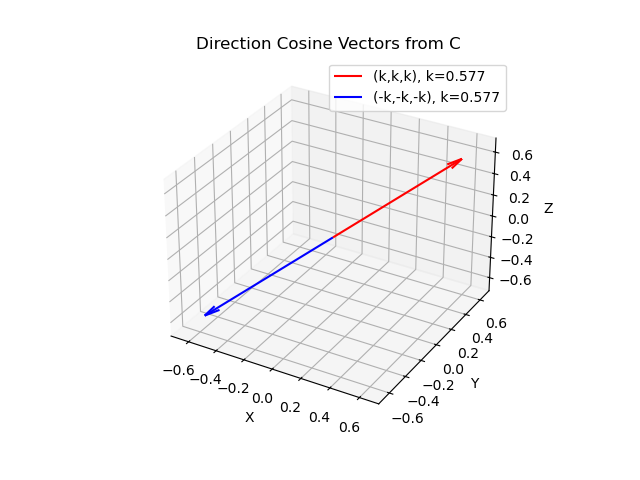
\includegraphics[width=0.7\columnwidth]{figs/Figure_1.png} 
   \caption*{Fig : PLOT BY SHARED OUTPUT}
  \label{Fig1}
\end{figure}

\begin{figure}[h!]
  \centering
  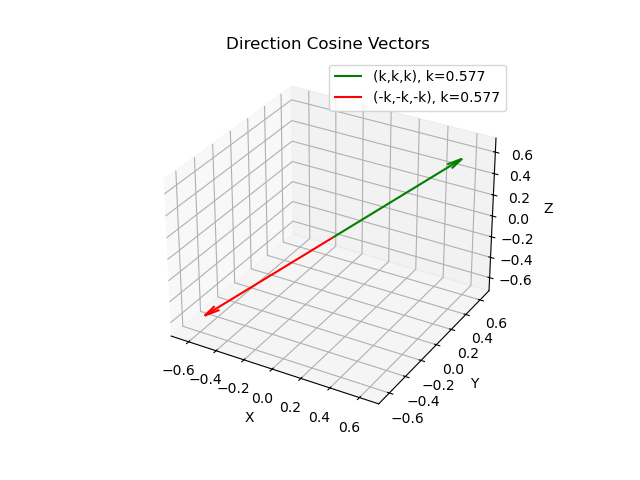
\includegraphics[width=0.7\columnwidth]{figs/Figure_2.png} 
   \caption*{Fig : PLOT BY DIRECT PYTHON CODE}
  \label{Fig2}
\end{figure}
\end{document}
